\section{MCMC Hammer \\(nonlinear model)}

Repeat problem 5.7 using either the
emcee package or by implementing your own slide-step sampler in place of the M-H sampler.
Make sure you clearly describe both your implementation as well as what checks you do to make sure that things have worked well.

\begin{figure*}
    \centering
    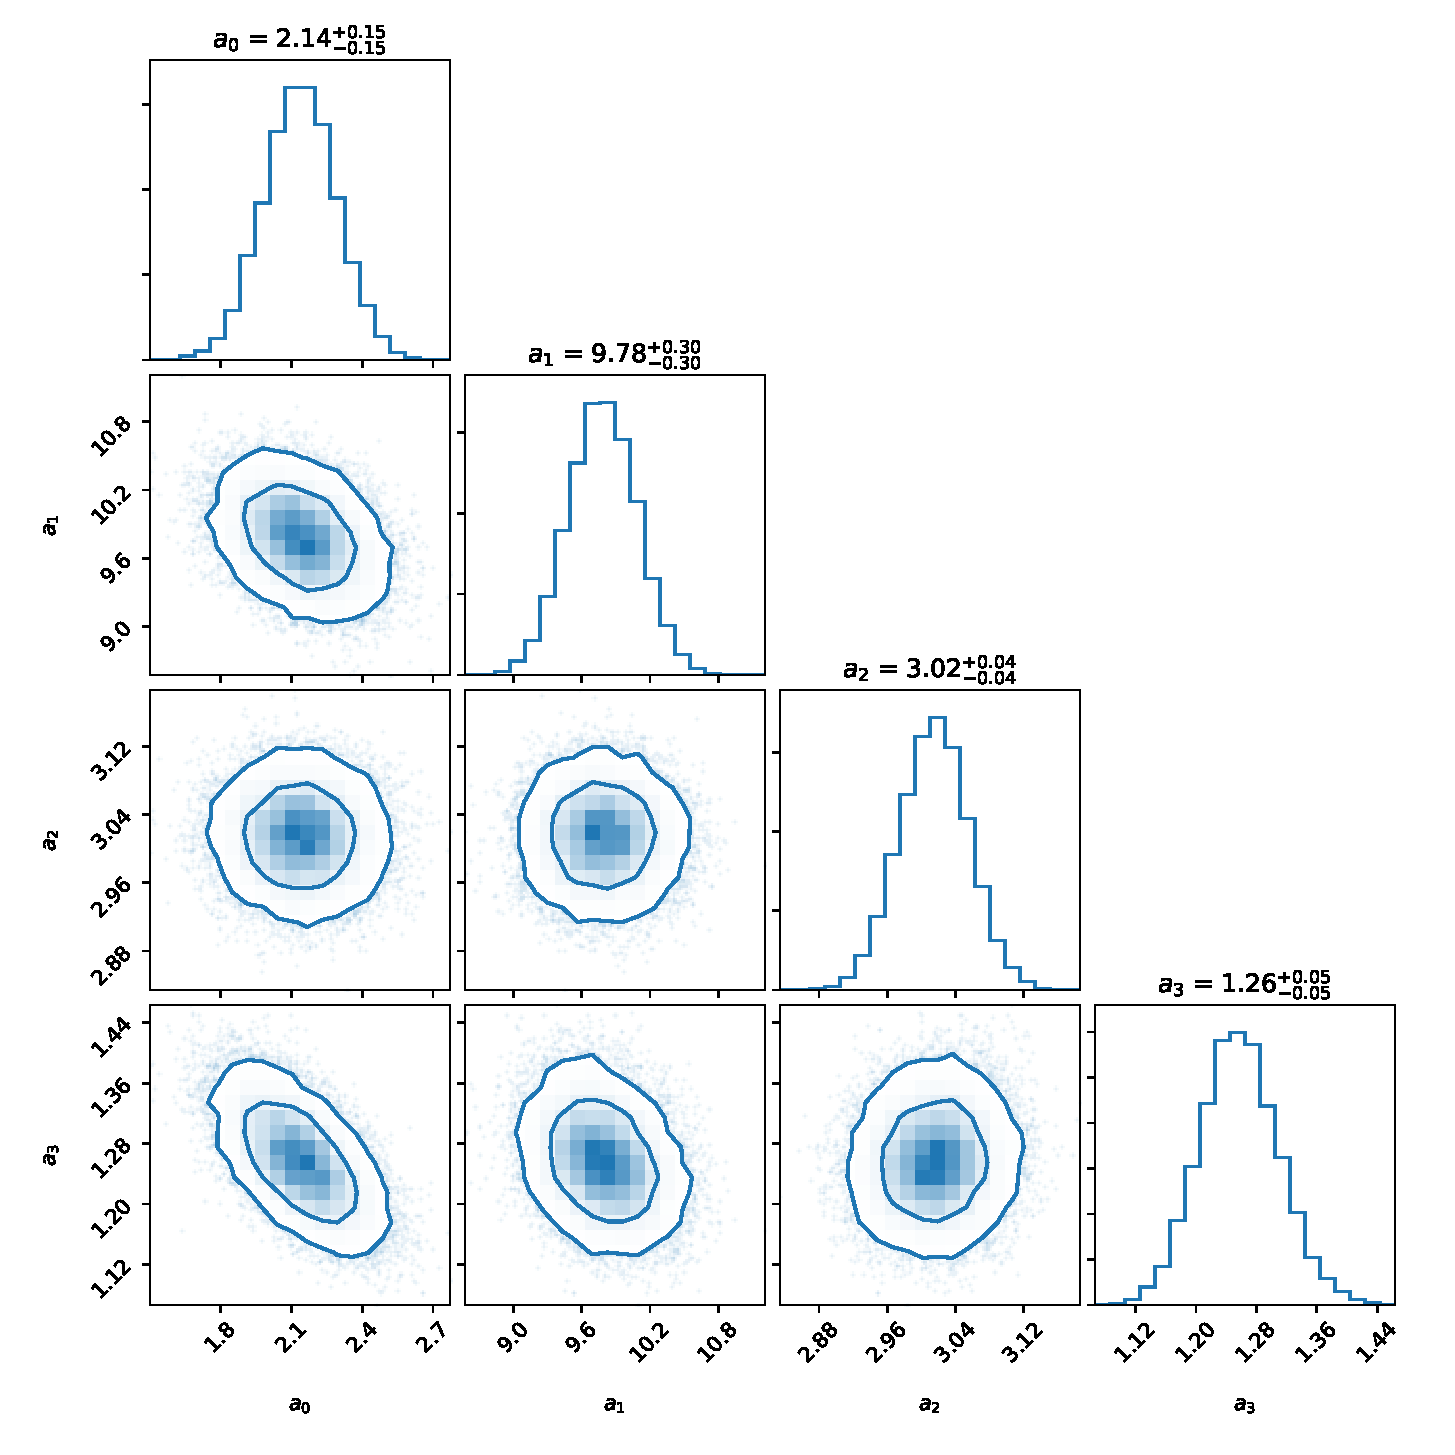
\includegraphics{CodeAndFigures/gaussianModelEmcee.pdf}
    \caption{Caption}
    \label{fig:gaussEmcee}
\end{figure*}